\documentclass{cph18}
\begin{document}

\section{Introduction}
   
Machine learning field approaches the creation of computer programm's that have the capability of automatically improve themselves through experience \citep{Michie1994,Levy1997,MacKay2005}. Classification techniques such as Euclidean and Mahalanobis similarity measurements are considered classical machine learning methods.  Those similarity measurements are referred to as distance attributes \citep{Deza2016}. Euclidean classifiers include a calculation of a centroid on the space of attributes. While the Mahalanobis takes into consideration the shape of attributes space. Both techniques are capable of making identification of geological cyclicity in data.

%Humanity uses their ability to recognize patterns since well before the dawn of the civilizatory process. Groups of Paleolithic humans recorded migratory patterns of certain groups of cervids. During the start of the Neolithic revolution, our ability to recognize patterns was directed to agriculture with the creation of monuments that registered the changes throughout the year. The human brain has evolved amazingly. And with regard to the quantity of information, the brain has an enormous advantage over the quantity of information processed by a computer \citep{Hall2014}. This does not stop only because some cells die. A computer does not function when its central processing unit is degraded \citep{Mao1996}.

%Artificial neural networks (ANN) are elaborated machine learning algorithm inspired by human brain \citep{Hagan1996}. Therefore an ANN is a mathematical algorithm that simulates tasks perfomed by a single neuron or a group of neurons. A neuron is the basic unit of an ANN \citep{Nedjah2016}. In a natural neural network, information pass through electrical impulses transmitted by synapses \citep{Krogh2008}. This work uses a special kind of ANN know as Self Organazing Map (SOM). 

A Self Organizing Map (SOM) is inspired by neural cortex \citep{Kohonen1989}. A SOM algorithm is based on a network \citep{Haykin2001}. This geometric arrangement is an oriented graph, whose vertices are the fundamental units know as artificial neurons and the edges are weights governing the interactions among neurons. Those artificial neurons change their weights as iteractions go on. 

%n the specific problem of logging wells, an important step is the identification of top and base layers that may be associated with changes in petrophysical properties \citep{Saljooghi2014}. Algorithms based on derivatives in the log curves do not identify very thin, or noisy layers \citep{Zhang1999}. \citep{Chakravarthy1999} can use the radial function to locate high-definition layer boundaries in induction log data (HDIL). However, \cite{Benaouda1999} can classify lithologic types into partially collapsed wells through the use of the neural network with error propagation and class changes as the analysis proceeds. \cite{Gloaguen2017} raises the question of the relative importance of physical properties in well profiling data for neural network decision making.

This work aims to define a comparison between a Kohonen SOM, an euclidean and a mahalanobean classificators. This comparison uses two well log data from a synthetic syneclises sedimentary basin type. It is remarkable that  the Mahalanobis classifier produced a higher error when compared to the Euclidean classifier and the SOM. The SOM presented better results for the two synthetic examples, with an error of $0.7$\% for the first well and $1.5$\% for the second. In contrast, Mahalanobis and Euclidean classifiers presented an error of $18.3$\% and $1.7$\% respectively for the first well and $11.3$\% and $6$\% for the second. 



\section{Methodology}
\label{Metodo}

In a general overview, the methodology adopted in this work is divided into three main parts. The first generates a synthetic syneclises sedimentary basin in which three synthetic wells are drilled (see Fig. \ref{Model}). The second part uses well log T$1$ to train the Kohonen SOM and obtain an optimal distribution of weights. Additionally, the same well is again used to store T$1$ log data into arrays. The last is to use the three techniques and compare the classified patterns for wells C$1$ and C$2$.

\subsection{Synthetic Sedimentary Basin}

The proposed model for the machine learning tests was based on a schematic geological model proposed by  \cite{Sal2008} for the Solim\~oes Sedimentary Basin, North part of Brazil. This modelling reproduces structures such as Horts, Grabens, normal and reverse faults. Fig. \ref{Model} shows the model with a zoom box highlighting the non-parallel contact of two differents lithotypes, where three wells were sampled. Four physical data properties were considered: density, gamma-ray, resistivity and velocity (see Tab. \ref{Tab1}). The sample rate for the well data is $0.01$ observation/meter with contamination of $5$\% gaussian noise.



\begin{figure}[ht]
	\centering
	\setlength{\fboxsep}{8pt}
	\setlength{\fboxrule}{0.1pt}
	\fbox{
	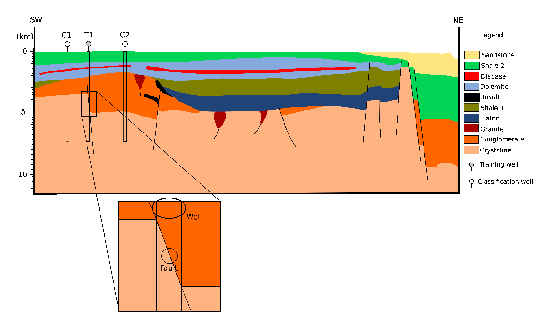
\includegraphics[scale=0.45]{Imagens/Basin.eps}
	}
	\caption{Synthetic Sedimentary Basin by \cite{Sal2008}  T1, C1 and C2 are training and classifing wells respectively.}
	\label{Model}
\end{figure}




\begin{table}[H]
\centering
\begin{tabular}{@{}ccccccccccc@{}}
\toprule
Rock & Density ($g/cm^{3}$) & Gamma-ray ($Ci/g$) & Resistivity ($\Omega/m$)& Velocity ($Km/s$) &\\ \midrule
Conglomerate &     $2.30$ 		  &       $100.0$       &           $6000$           &			$2$   		   	&\\
Shale	 &       $2.55$           &       $100.0$       &           $1000$           &     		$3$		 &\\
Dolomite     &       $2.72$           &       $8.30$        &           $3.5 \times 10^{3}$           &  	$6$    			 &\\
Diabase    &       $2.91$           &       $30.0$        &           $15 \times 10^{7}$           &      $5.5$				 &\\
Crystalline  &       $2.80$           &       $0.7$         &           $1.3 \times 10^{6}$           & 		$5$		     &\\ \bottomrule
\end{tabular}
\caption{Physical properties.}
\label{Tab1}
\end{table}

%Fig. \ref{C3} shows the synthetic well and it distribution of geophysics properties along diferents rocks.  

\subsection{Training and Similarities}

SOM are machine learning types composed by oriented graphs that are distributed on a hyperplane inside a hyperspace of features.  Features are the physical properties that are correlated with a specific type of rock. The identification process is based on redundance of patterns. A toroid geometry is adopted here for the SOM with $400$ neurons.  Vector \textbf{X} is composed of physical properties from the training well T1 with dimension $n$, where $n$ is the number of data. \textbf{X} is related to a neuron with a $w_{i,j}$ weight matrix, as follows:    

\begin{figure}[H]
	\centering
	\setlength{\fboxsep}{8pt}
	\setlength{\fboxrule}{0.1pt}
	\fbox{
	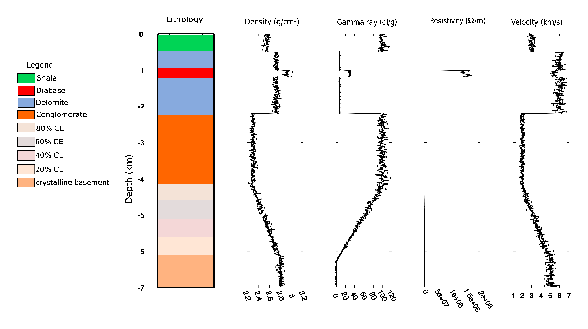
\includegraphics[scale=0.5]{Imagens/T1130118.eps}
	}
	\caption{Synthetic training well T$1$. The normal fault was created by four divisions on the range of the normal fault, decreasing the amount of conglomerate in comparison to cryshalline basement. That behavior simulates a special kind of logging signature. }
	\label{C3}
\end{figure}



%\begin{displaymath}
% \mathbf{X}=\left(\begin{array}{r}
%x_{1}\\
%x_{2}\\
%x_{3}\\
%  \vdots \\
%x_{m}
% \end{array}\right)
% \end{displaymath}

\begin{eqnarray}
d(t)= \sqrt{\sum^{n}_{i=1}[x(t)-w_{i,j}(t)]^{2}} \hspace{1cm}  (j = {1,..,m}), %\nonumber
\label{eq1}
\end{eqnarray}
 where $t$ is the number of iterations, $x(t)$ is an element of \textbf{X} and $d(t)$ is the metric. The lowest value of $d(t)$ defines the best neuron for a specifc attribute.
 
 
 % This neuron changes the value of the surrounding neurons inside the quartet geometry according to the Eq. \ref{eq2}.

%\begin{equation}
%w_{i,j}(t+1)=w_{i,j}(t)+\eta(t)[x(t)-w_{i,j}(t)] 
%\label{eq2}
%\end{equation}  
%
%Where $w_{i,j}(t+1)$ is the updated weight matrix and $\eta(t)$ is the learning rate. The learning rate is the measurement of how fast does the algorithm learn, Eq. \ref{eq3}.

%\begin{equation}
%\eta(t)=\eta(0)    ( 1 -  \frac{t}{T}  ) 
%\label{eq3}
%\end{equation}  
%
%Where $T$ is the number of training cyles and $t$ is the number of iteractions. A iteractive process $t=t+1$ goes on until $t \approx  T$. Once the process ends for one neuron it repeats it self for the surrounding neighbors.

The Euclidean classifier is a statistical non-parametric classifier that uses the same input vector  $\textbf{X}$ for its training process. A mean vector $\bar{\textbf{X}}_{i}$ for each property is calculated and stored in a set of training $i$. Then the Euclidian distance for the $i$-th set ($Ed_{i} $) is computed as the following:

\begin{equation}
Ed_{i} =  \Arrowvert \textbf{X}-\bar{\textbf{X}}_{i}  \Arrowvert^{\frac{1}{2}}, 
\label{eq4}
\end{equation}  
where \textbf{X} is the set of physical properties to be classified. 

The Mahalanobis Classifier computes the mean vector $\bar{\textbf{X}}_{i}$ and the covariance matrix $\textbf{C}_{i}$ for each ensemble. The Mahalanobis distance ($Md_{i}$) is computed as:


\begin{equation}
Md_{i}=[(\textbf{X}-\bar{\textbf{X}}_{i})^{T}\textbf{C}_{i}^{-1}(\textbf{X}-\bar{\textbf{X}}_{i})]^{\frac{1}{2}}.
\label{eq5}
\end{equation}

The covariance matrix is defined as:

\begin{equation}
\textbf{C}_{i}=\frac{1}{n_{i}-1}\sum_{X \in \omega_{i}}(\textbf{X}-\bar{\textbf{X}}_{i})(\textbf{X}-\bar{\textbf{X}}_{i})^{T}
\label{eq6}
\end{equation}


\section{Results}
\label{Resultados}
Fig. \ref{C1} (A) shows the original well. Fig. \ref{C1} (B), (C) and (D) present the final classification for SOM, Euclidean and Mahalanobis. All errors were concentrated on a single lithotype, the crystalline rock. Those errors indicate $11$ swaping between crystalline rock and $20\%$CE rock type for the SOM classificator.    

\begin{figure}[H]
	\centering
	\setlength{\fboxsep}{8pt}
	\setlength{\fboxrule}{0.1pt}
	\fbox{
	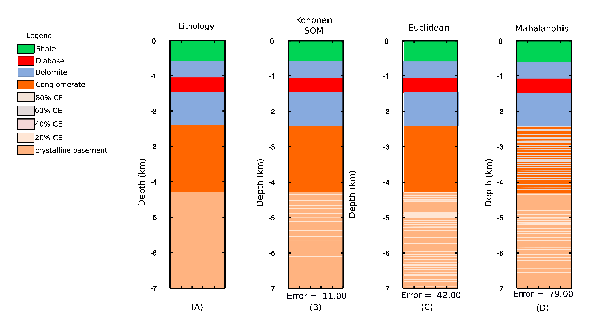
\includegraphics[scale=0.5]{Imagens/IDC1020118.eps}
	}
	\caption{Comparison between the classificators and SOM for C1 well data. }
	\label{C1}
\end{figure}

Euclidean classificator results on $42$ errors. Those errors present the same pattern of SOM classificators. Mahalanobis classificator shows $79$ errors. It misjudgeds the crystalline rock data with the $20\%$CE rock and the conglomerate with the $60\%$CE rock. 

Fig. \ref{C2} (A) shows the synthetic well. Fig. \ref{C2} (B), (C) and (D) present the comparison among the three methodologies.  In a overall perspective, SOM shows better results. Again for the three methods, the major misleading occurs in the classification of crystalline basement.  

\begin{figure}[H]
	\centering
	\setlength{\fboxsep}{8pt}
	\setlength{\fboxrule}{0.1pt}
	\fbox{
	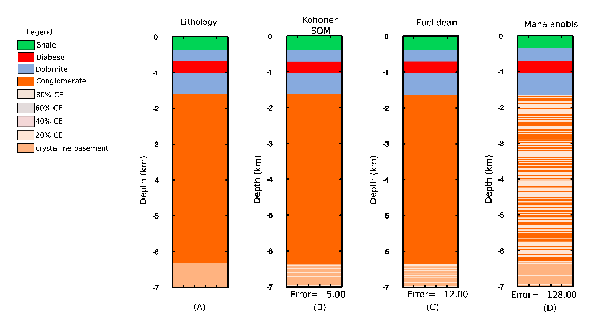
\includegraphics[scale=0.5]{Imagens/IDC2020118.eps}
	}
	\caption{Comparison between the classificators and SOM for C2 well data. }
	\label{C2}
\end{figure}

\section{Conclusions}

Two synthetic tests of well logging were performed to understand the behavior of three different machine learning elements: Kohonen SOM, Euclidean and Mahalanobis classificators. As expected, the SOM overperformed the classificators due to a more detailed algorithm. On the other side, the computational requirements for SOM are more demanding than the classificators, which indicates that the choice of the method depends on the number of data sets.   

As perspectives, we are intended to apply these methods to more complex synthetic scenarios and also with real data acquired on Paran\'a Sedimentary Basin, South portion of Brazil. 

%Fig. \ref{C1} ilustrates that all the three methodologies confused crystalline basement with $20\%$CE rock. This first observation occurs due to a diffuse dispersion between these two types of rock inside the hyperspace of characteristics. It shows a reflection of the choice of training well log data. Mahalanobis classificator also interchanges congolerate with $60\%$CE, indicating difficulties to indetify this rock unit. 

%Fig. \ref{C3} located in a normal geological fault. This type of structure creates a mixture between the physical properties of the rocks in the fault range within the well environment.

%Fig.\ref{C2} shows the same kind of behavior regarding interchages on cristalline basement and $20\%$CE, and conglomerate and $80\%$CE. The numbers of errors increases on the C$2$ site for mahalanobis classifier. That behavior is related to the decrease of crystalline rock on C$2$ well. 

 

%This natural arrangement means that the mahalanobis classifier did not perform as well as expected. In contrast the euclidean classifier shows a better relative performace. That occurred because euclidean classificator computes the centroid inside the hyperspace of attributes. 

%This simulation indicates that Self Organizing Maps had the best performance in comparison to he Classificator's methodology.  


%\bibliographystyle{authordate4}
  \bibliography{references}
  
\end{document} 
